%% OfficeFloor - http://www.officefloor.net
%% Copyright (C) 2013 Daniel Sagenschneider
%%
%% This program is free software: you can redistribute it and/or modify
%% it under the terms of the GNU General Public License as published by
%% the Free Software Foundation, either version 3 of the License, or
%% (at your option) any later version.
%%
%% This program is distributed in the hope that it will be useful,
%% but WITHOUT ANY WARRANTY; without even the implied warranty of
%% MERCHANTABILITY or FITNESS FOR A PARTICULAR PURPOSE.  See the
%% GNU General Public License for more details.
%%
%% You should have received a copy of the GNU General Public License
%% along with this program.  If not, see <http://www.gnu.org/licenses/>.
%%
%% While this document is not a program, it conveys the underlying design 
%% of OfficeFloor (it is the expression of how to implement the ideas of 
%% Thread Injection, Implicit Thread, Continuation Injection, Operation 
%% Orchestration, Inversion of Control) and as such any program derived from 
%% the contents (expression) of this document is considered conveying 
%% (copying/modifying) the OfficeFloor expression and is therefore subject 
%% to the licensing of OfficeFloor.




%%This is a very basic article template.
%%There is just one section and two subsections.
\documentclass[prodmode]{style/acmlarge}

% Include packages
\usepackage{listings}
\usepackage{caption}


% Metadata Information
\acmVolume{V}
\acmNumber{N}
\acmArticle{A}
\articleSeq{S}
\acmYear{YYYY}
\acmMonth{0}

% Package to generate and customize Algorithm as per ACM style
\usepackage[ruled]{style/algorithm2e}
\SetAlFnt{\algofont}
\SetAlCapFnt{\algofont}
\SetAlCapNameFnt{\algofont}
\SetAlCapHSkip{0pt}
\IncMargin{-\parindent}
\renewcommand{\algorithmcfname}{ALGORITHM}

% Page heads
\markboth{D. Sagenschneider}{OfficeFloor: using office patterns to improve software design}


\title{OfficeFloor: using office patterns to improve software design}
\author{DANIEL SAGENSCHNEIDER \affil{OfficeFloor, daniel@officefloor.net}}

\begin{abstract}
OfficeFloor is a middleware framework that bases its design on the patterns
occurring within the office.  Re-using office patterns within software enables
improved performance tuning of applications operating within complex enterprise
environments and enables earlier and continuous delivery of working code for
Agile methodologies.  The improved performance tuning uses multiple thread pools
to isolate the performance impacts of the application in interacting with
multiple downstream systems (e.g. an application operating in a complex
enterprise environment, such as Service-Oriented Architecture).  The earlier and
continuous delivery of working code is enabled by inversion of control.
OfficeFloor is a middleware framework that provides inversion of control for
methods to build applications bottom-up.  The bottom-up approach to building
applications reduces the lead times and reduces the refactoring of top-down
software designs to enable early and continuous delivery of working code for
Agile methodologies.
\end{abstract}

\category{D.2.11}{Software Architectures}{Patterns}
\category{D.2.3}{Coding Tools and Techniques}{Object-oriented programming}
\category{D.2.6}{Programming Environments}{Graphical environments}

\terms{Design, Performance, Standardization}
\keywords{Inversion of Control, Responsible Thread Pool, Task Orchestration}

\acmformat{Sagenschneider, D. 2013. OfficeFloor: using office patterns to improve software design.}

\copyr{Copyright 2013 is held by the author}

\begin{document}

% Configure Graphics package
\graphicspath{{./pdf/}}
\DeclareGraphicsExtensions{.pdf}

% Configure Listings package
\lstset{language=Java}

% Configure Captions package (listing small font)
\captionsetup[lstlisting]{font=footnotesize}


\begin{bottomstuff}
This work is the result of the author's development of OfficeFloor.\\
Author: D. Sagenschneider; email: daniel@officefloor.net\\

Permission to make digital or hard copies of all or part of this work for
personal or classroom use is granted without fee provided that copies are not
made or distributed for profit or commercial advantage and that copies bear this
notice and the full citation on the first page. To copy otherwise, to republish,
to post on servers or to redistribute to lists, requires prior specific
permission. A preliminary version of this paper was presented in a writers'
workshop at the 18th European Conference on Pattern Languages of Programs
(PLoP).
\end{bottomstuff}

\maketitle


%% TODO before final draft:
%%   - confirm SEDA adds/removes threads


\section{Introduction}

OfficeFloor~\cite{officefloor} is a middleware framework that models its
architecture on patterns occurring in offices.  The premise of this modelling is
that business processes occurred manually within offices before technology
systems began automating tasks.  Therefore, rather than impose mechanical
software models on the business
\cite{enterprise-process-modelling,model-business-process,model-sociotechnical},
this paper discusses OfficeFloor's use of office patterns occurring within
businesses to improve software design.

The patterns presented in this paper are the result of the author's translation
of observed office patterns into software design to create the OfficeFloor
middleware framework.  Patterns provide solutions to re-occurring problems
\cite{pattern-language}.  The problem of an office interacting with multiple
external parties (e.g. customers, suppliers, service providers, other offices)
is a similar problem to an application interacting with multiple external
systems (e.g. Service-Oriented Architecture).

The use of the office solutions within this paper addresses two problems within
software design.  The first software problem is to enable performance tuning of
an application to operate in a complex enterprise environment that requires
interaction with many downstream systems \cite{reverse-ten-k-problem}.  The
second software problem is providing a technical framework that enables
delivering working software earlier and continuously \cite{agile-manifesto}.

\begin{figure}[!t]
\centering
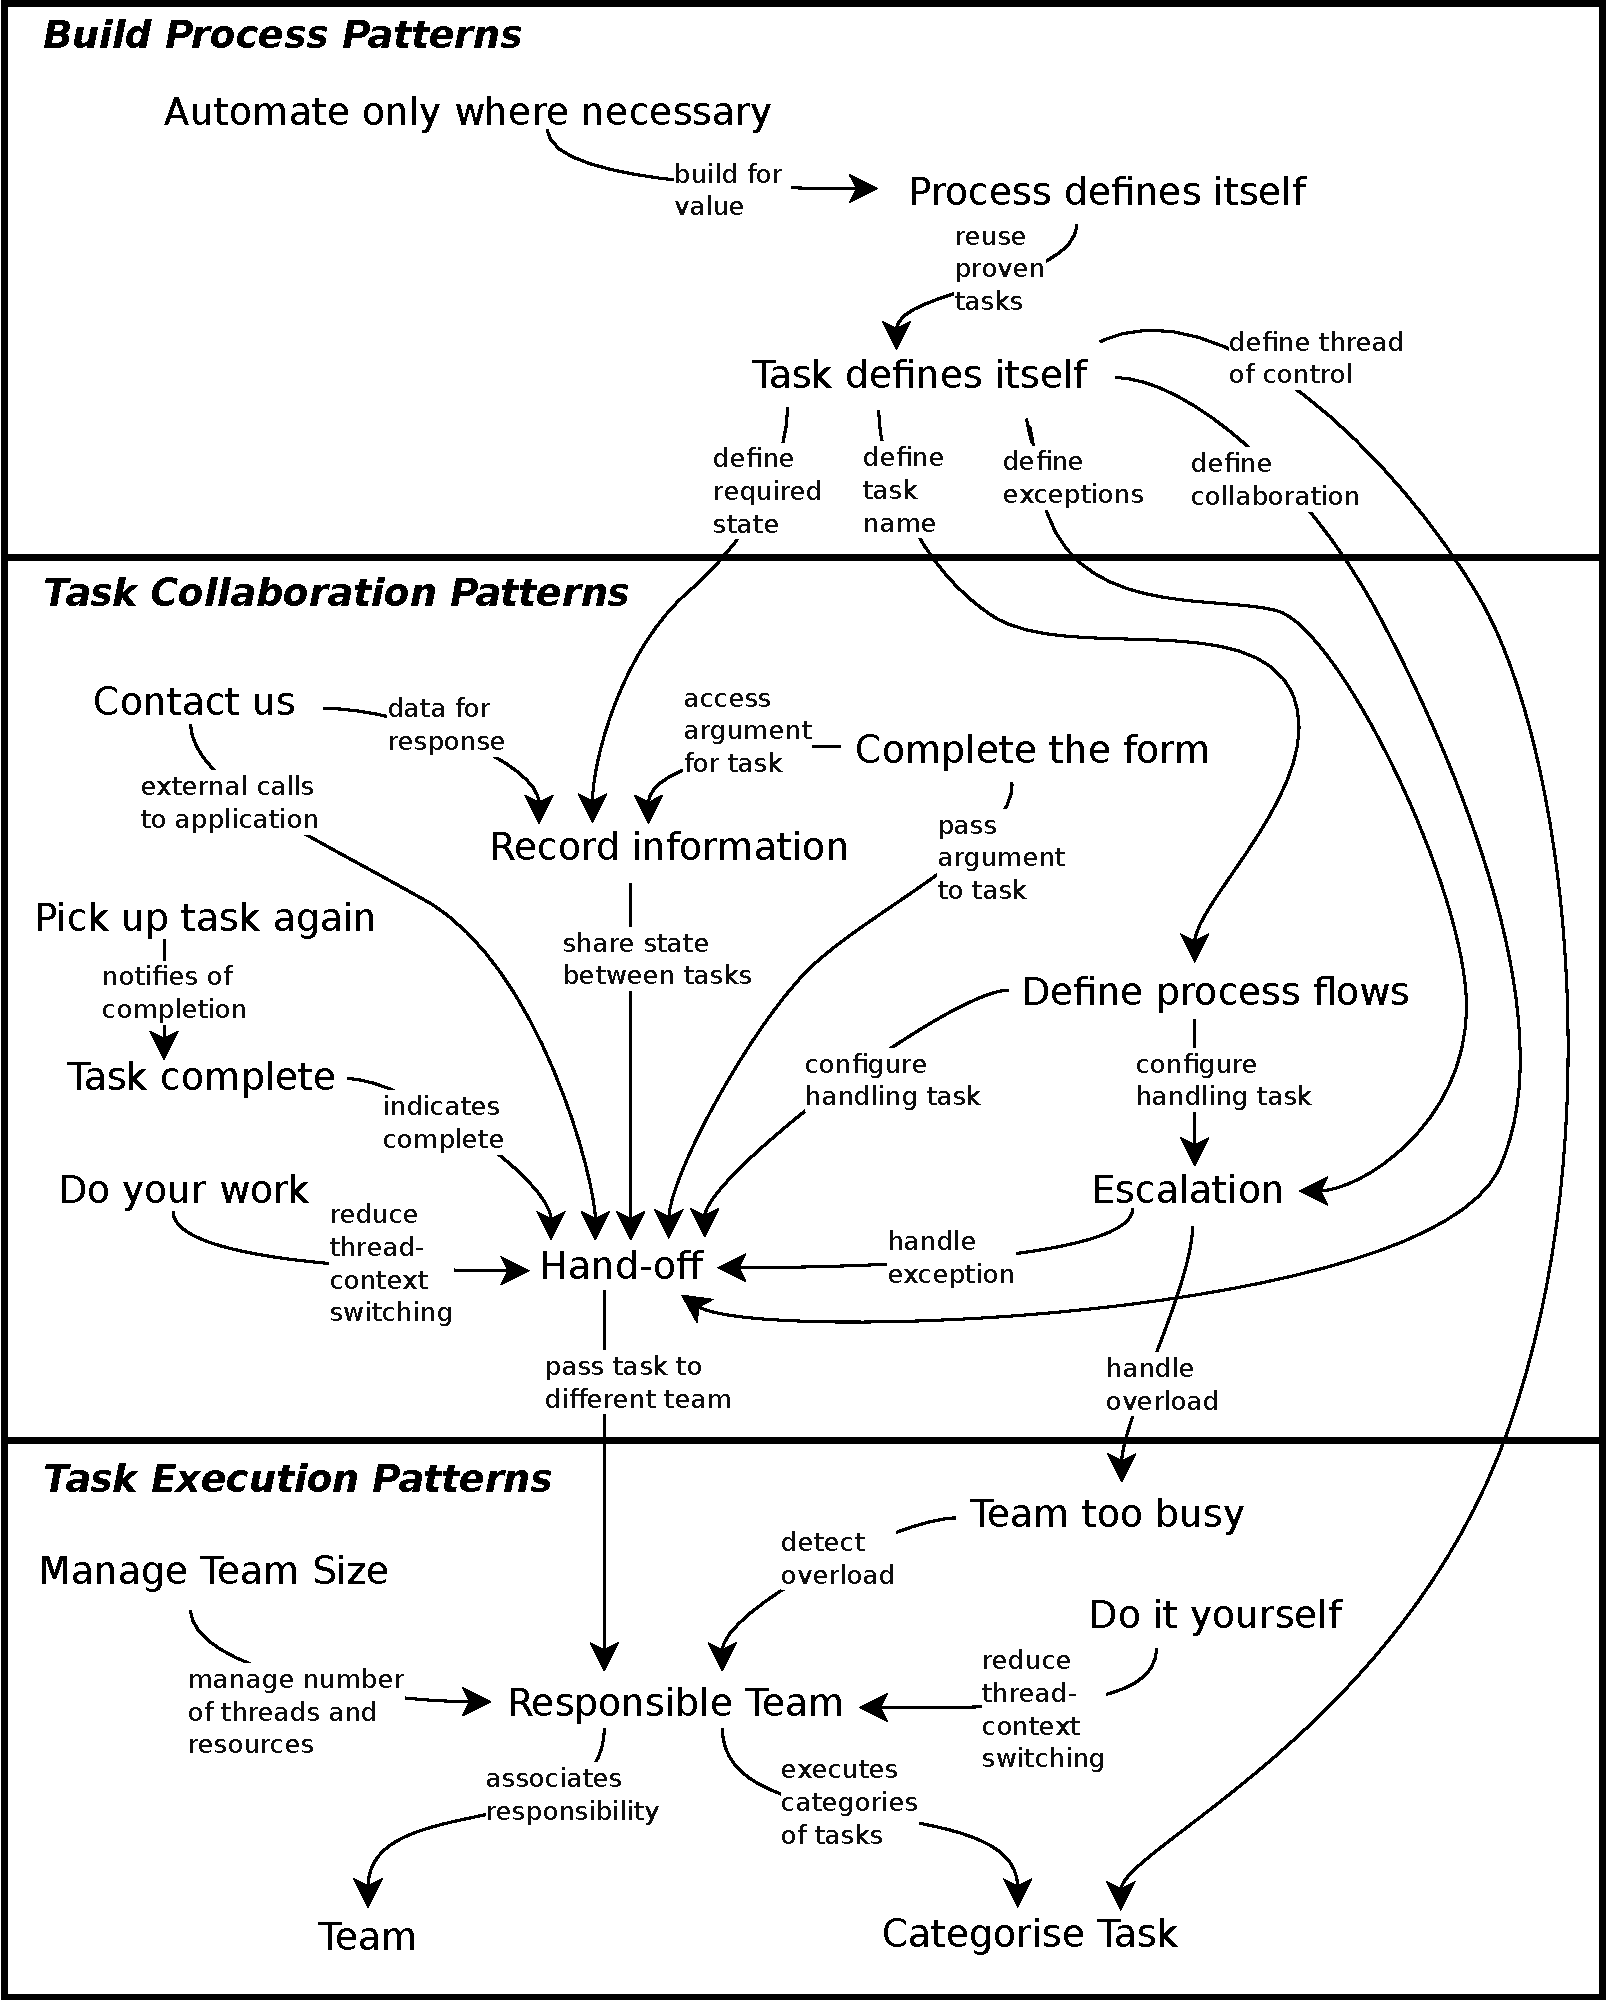
\includegraphics[height=7.4in]{PatternRelationships}
\caption{Relationships of the patterns presented in each section of this paper.}
\label{fig:PatternRelationships}
\end{figure}

To re-use the office solutions for software problems, software concepts need to
be mapped to office concepts.  This enables the office patterns to be used in
software design.  The following analogies are made by the author to enable
re-using office patterns for software design:
\begin{description}
  \item[Thread] is mapped to the concept of a Person (Worker),
  \item[Method] is the functionality of a Task (activity/step of a process),
  \item[Component] is similar to a Process (as both contain composite functionality),
  \item[Object fields] is the structured information managed within an office (e.g. form),
  \item[Application] is similar to an Office (manages information and undertakes decisions).
\end{description}

In using the office patterns for software design, many of the offices issues do
not occur in software.  The organisation structure and behaviour within an
office must account for people \cite{organisational-behaviour}.  Within software
the people aspects do not need consideration.  The thread (person) will
mechanically undertake all methods (tasks) exactly as specified.  Therefore, in
following the above analogies, the grouping of threads into thread pools is
similar to grouping people into functional teams\footnote{The use of the term
team within this paper more closely aligns to staff of a functional department.
However, the author finds the term department is perceived as more than just the
staff.  The author, therefore, uses the term team as a better analogy to focus
the reader on a thread pool being a group of threads (people) with the goal of
completing a set of related methods (tasks).  Also, the \textsc{do it yourself}
pattern does enable a thread pool (team) to execute methods (tasks) outside its
responsible category (functional departmentalisation).}.  Each team (thread
pool) will undertake a specific set of tasks (methods) exactly as specified.

The patterns presented in this paper are discussed in three sections.  These
sections present the patterns for execution of tasks, collaboration
of tasks, and building processes from tasks.  Figure
\ref{fig:PatternRelationships} shows the relationships between the patterns
presented in each section of this paper.  Each section is written in two parts.
The first part lists the office patterns and how they influence change in
software design.  The second part of each section provides notes on
OfficeFloor's implementation of the patterns as a middleware framework.  This
paper assumes knowledge of existing software design only for the implementation
notes.  The implementation notes may be skipped by those readers only interested
in the influence of the office patterns on software design.



\section{Patterns for execution of tasks}

The following patterns model the execution of methods on the way tasks are
undertaken within an office.  These patterns address the first software problem
addressed by this paper - performance tuning an application to operate within a
complex environment.  The implementation notes at the end provide details on how
to implement the combined patterns.


\subsection{\textsc{\textbf{team}}}

\subsubsection*{Context} Within an office, work loads can far exceed that
possible by a single person. This is resolved within an office by creating a
team of people to concurrently undertake the tasks.

Within software, developers write code of a method (task) for a single thread
(person).

\subsubsection*{\textbf{Problem}} Improving throughput of executing many methods.

\subsubsection*{Forces} Developer writes intuitive sequential code.

\subsubsection*{\textbf{Solution}} Use a pool of threads to execute the methods
concurrently.

\subsubsection*{Consequences} Having more people allows getting more tasks done.
Similarly having more threads allows more methods to be executed.

The people in an office need to coordinate so the tasks get done correctly and
efficiently.  This is similar to the concurrency issues occurring in executing
methods concurrently.

\subsubsection*{Related patterns} Also known as \textsc{thread pool}~\cite{thread-per-request}.

\subsubsection*{Notes} The \textsc{team} pattern is provided as an example to
demonstrate how the analogies in the introduction enable re-use of the office
patterns. See the \textsc{thread pool} pattern~\cite{thread-per-request} for a
detailed explanation of this pattern.



\subsection{\textsc{\textbf{categorise task}}}

\subsubsection*{Context} Within an office, to assign a task to a particular team
a description of the task is required to identify which team is responsible for
undertaking the task.  This description allows categorising similar tasks
together.  Each grouping of similar tasks are then undertaken by a particular
team for improved efficiencies.  For example, a financial task is undertaken by
the finance team.

Within software, methods (tasks) are associated to objects/classes and are not
categorised.

\subsubsection*{\textbf{Problem}} Providing a description of the method for it to be
categorised into a group of related methods.

\subsubsection*{Forces} The method name is free text and is unlikely to follow a
naming convention that allows parsing out the method's category.  Furthermore, the
developer should not have to write the description of the method.

\subsubsection*{\textbf{Solution}} Use the parameter types of the method to categorise
the method.  For example, all methods that declare a database connection
parameter are grouped into a category of tasks that are interacting with the
database.

For finer grained categorisation, use annotations on the parameter types.

\subsubsection*{Consequences} The method name is not required for categorising.
Also, the developer is not required to provide any more details except the
parameters the method requires.  However, methods that have unused parameters
may be incorrectly categorised.

\subsubsection*{Related Patterns} \textsc{responsible team} provides the thread
pools to execute the categories of methods.



\subsection{\textsc{\textbf{responsible team}}}

\subsubsection*{Context} Within an office, there are different teams responsible
for the differing categories of tasks within the process.  For example, the
financial team will do the finance tasks and the software development team will
do the software development tasks.  Assigning particular teams to each category
of tasks allows specialising the teams to their tasks.

Within software, thread pools (teams) execute any methods (tasks) they are
assigned.

\subsubsection*{\textbf{Problem}} Making the thread pool responsible for a particular
category of methods.

\subsubsection*{Forces} The thread pool name is free text and is unlikely to
follow a naming convention that allows parsing out the thread pool's responsible
task categories.  Furthermore, the developer should not have to provide code to
make decisions over thread pool responsibilities.

\subsubsection*{\textbf{Solution}} Configure each thread pool with an attribute
containing the type that defines its responsible category of
methods\footnote{The thread pool may be configured with more than one type to be
responsible for multiple categories of methods.}. Methods are then executed by
the thread pool whose responsibility type matches one of the method's parameter
types (\textsc{categorise task} types).  A default thread pool is used if no
match occurs.

For example, configure the thread pool responsible for all database interaction
with the database connection type.  As each method is categorised by the
\textsc{categorise task} pattern, all methods requiring a database connection
are executed by this thread pool.

\subsubsection*{Consequences} There will always be a thread available in each
thread pool to execute their respective responsible category of methods. 
Subsequently, if there is a significant increase in the number of methods in one
category all threads do not become focused on these methods to the detriment of
the other categories of methods.

The threads in each thread pool are also specialised based on their responsible
category of methods (e.g. change in nice value, affinity to CPU).  However,
threads may be idle if no methods occur for their responsible category.

\subsubsection*{Related Patterns} Is a sequence on \textsc{team} to identify
the responsible categories of methods to execute.



\subsection{\textsc{\textbf{manage team size}}}

\subsubsection*{Context} Within an office, as the number of tasks for a
responsible team grows or shrinks, the size of the team is altered to obtain
optimal throughput.  For example, near the end of the financial year the finance
team will be increased in size for the additional number of financial year end
tasks.  The software development team, however, would not be changed in size as
the development tasks stay the same in number.

Within software, the thread pool (team) controls the number of threads (people)
to execute methods (tasks).

\subsubsection*{\textbf{Problem}} Obtain optimal throughput execution of methods by a
thread pool.

\subsubsection*{Forces} Having too few threads will under utilize the hardware
and not provide optimal throughput.  Having too many threads will cause
excessive thread-context switching and exhaustion of available resources (e.g.
memory), which in turn will decrease throughput.

\subsubsection*{\textbf{Solution}} As each \textsc{responsible team} thread pool
is responsible for a particular dependency (resource), use adaptive resource
management~\cite{seda} to manage the number of threads within each responsible
thread pool.

Adaptive resource management (from the Staged Event Driven Architecture
\cite{seda}) monitors the number of tasks and their execution time and
adds or removes threads and resources to achieve optimal throughput by the thread
pool (stage).

\subsubsection*{Consequences} The thread pool size will dynamically grow or
shrink based on its load of responsible methods to execute.  However, this does
require a small overhead in monitoring the execution of methods.

\subsubsection*{Related Patterns} Is a sequence on \textsc{responsible team} to
manage the thread pool size.



\subsection{\textsc{\textbf{do it yourself}}}

\subsubsection*{Context} Within an office, certain tasks are more efficient if
undertaken by oneself without delegating to someone else.  If every task along
the process had to be undertaken by a different person, it would create
significant communication overheads, which would negatively impact the
efficiency of the office.  Therefore, within an office many tasks are undertaken
by the current person involved in the process.

Within software, assigning a method (task) to a thread pool (team) requires an
effective thread-context switch to execute the method.  Having to thread-context
switch for execution of each method is inefficient and will degrade performance
of the application.

\subsubsection*{\textbf{Problem}} Avoid thread-context switching to execute each method.

\subsubsection*{Forces} Each category of methods will be executed by a
particular responsible thread pool.  Stepping between these categories results
in the use of different responsible thread pools, which requires a
thread-context switch.  However, it is cheaper to execute many methods in the
process using the current thread of control than incur the cost of a
thread-context switch (i.e. easier to do yourself).

\subsubsection*{\textbf{Solution}} Use a responsible thread pool that has no threads.
The method is executed immediately by the thread of control that registers the
method with the thread pool (i.e. borrows the thread of control).

\subsubsection*{Consequences} Categories of methods are executed by the calling
thread of control and subsequently do not incur a thread-context switch.
However, this does enable incorrectly categorised methods to potentially cause
thread starvation of the wrong thread pool.

\subsubsection*{Related Patterns} Is a sequence on the \textsc{responsible team}
to reduce thread-context switching.  It is also similar to the \textsc{reactor}
pattern~\cite{reactor} in reusing the thread of control.



\subsection{\textsc{\textbf{team too busy}}}

\subsubsection*{Context} Within an office, when there is a very large number of
tasks to complete, teams will not be able to complete all their tasks within the
required period of time.  The teams may be increased in size to cope with the
additional tasks.  However, at a certain point there are too many tasks and the
team will not take on new tasks.

Within software, the thread pool (team) queues methods (tasks) for execution
when all its threads (people) are busy.  At a certain point the queue length
will grow to a point where new methods added to the queue will not be executed
within a reasonable period of time.

\subsubsection*{\textbf{Problem}} Stop the thread pool taking on new methods so
it may cope with the current load of methods.

\subsubsection*{Forces} The thread pool will execute all methods added to its
queue.  When the number of methods registered for execution is continually more
than the number of methods able to be executed, the queue grows.  At a certain
point the time between registering a method and the actual execution of the
method is so large that the resulting method execution is no longer relevant. 
Execution of these methods then results in wasted use of threads and a
non-responsive application.

\subsubsection*{\textbf{Solution}} Use admission control~\cite{seda} for each
responsible thread pool.  At a certain queue size admission control will
disallow further methods from being registered.

The responsible thread pool will execute all methods that are registered.  For
methods not registered, \textsc{escalation} enables alternate methods to be
undertaken by other less busy thread pools (e.g. for a web server this could be
responding with a server temporarily busy page).

\subsubsection*{Consequences} Not registering methods for execution during
overload of the server does result in methods not being executed.  However,
overload of the server does require actions to be undertaken to deal with the
overload.  Not taking action will result in exhausted resources of the server
and potential for the application to crash (e.g. exhaust available memory).

\subsubsection*{Related Patterns} Is a sequence on \textsc{responsible team} to
handle overload of methods for a responsible thread pool.  \textsc{escalation}
is used to handle methods not registered for execution.



\subsection{\textbf{Implementation notes for the task execution patterns}}

\subsubsection*{Background}

Both the \textsc{thread-per-request} pattern \cite{thread-per-request} (basis of
many mainstream middleware designs\footnote{Example middleware using
\textsc{thread-per-request} is the popular web servers (Netcraft November 2012
survey) that serve dynamic web content by CGI/FastCGI with for example PHP scripts,
Microsoft's HTTP.sys/WAS, and JEE Servlets.}) and the \textsc{proactor} pattern
\cite{proactor} (basis of event-driven middleware designs) enable a different
thread of control for the execution of a request/task.  These patterns allow for
concurrent execution by utilising many threads.  For efficiencies the
\textsc{thread pool} pattern \cite{thread-per-request} is commonly used to pool
threads to reduce thread management overheads.

As identified by the \textsc{proactor} pattern, the threading ``must be designed
carefully to support prioritization and cancellation'' \cite[p. 8]{proactor} of
the execution of tasks.  However, both the \textsc{thread-per-request} pattern and
the \textsc{proactor} pattern do not define algorithms for
prioritisation and cancellation of tasks and leaves this to the developer.

Isolation of tasks is necessary to reduce trade-offs in performance tuning. 
Utilising a single pool of threads to service all requests results in tuning
trade-offs, which degrades performance of the server during particular load
profiles (e.g. high load of requests blocked on database I/O that are starving
requests for cached data of a thread).  This is further evident in the
performance analysis of web servers which identifies the importance of tuning
the server for a load profile
\cite{tuning-important,low-server-footprint,tuning-os-important}.

Having an ability to cancel tasks is important to avoid overloading the server.
As load increases on the server, the resources available will be exhausted
causing delays in servicing requests and in some scenarios cause the server to
crash (e.g. exhausting available memory).  Tasks must be cancelled to reduce the
load on the server.  However, only tasks causing bottlenecks should be cancelled
(e.g. a request for cached data should not be cancelled if it is the database
that is overloaded).


\subsubsection*{Implementation}

The \texttt{Task} (Listing \ref{lst:TaskExecutionInterfaces}) is the object that wraps
the method to provide a standard interface for execution of methods.  This
enables for a single \texttt{TaskExecutor} implementation (Listing
\ref{lst:TaskExecutionInterfaces}) to execute differing methods.

To execute a method the client code invokes \texttt{executeTask(\ldots)}
(Listing \ref{lst:TaskExecutionInterfaces}) with the identifier of the desired
\texttt{Task} (method).  The \texttt{TaskExecutor} uses the
\texttt{DependencyInjectionFactory} to construct the \texttt{Task}
and the dependencies for the \texttt{Task} (i.e. the parameters for the method
wrapped by the \texttt{Task}).  The \texttt{TaskExecutor} then assigns the
\texttt{Task} for execution by one of the many developer configured thread pools
(\textsc{team}).  Figure \ref{fig:ExecuteComponentSequenceDiagram} provides a
sequence diagram of executing a \texttt{Task}.

\lstset{caption=Task execution pattern interfaces.  The task collaboration patterns in the next section build on these interfaces to enable collaboration of the \texttt{Task}s.}
\begin{lstlisting}[float,label=lst:TaskExecutionInterfaces]

    interface Task {
        void execute(); 
        void cancel(Exception cause);
    }

    interface TaskExecutor {
        void executeTask(String taskId);
    }

    interface DependencyInjectionFactory {
        Task createTask(String taskId);
        Type[] getRequiredDependencyTypes(String taskId);
    }
\end{lstlisting}


\begin{figure}[!t]
\centering
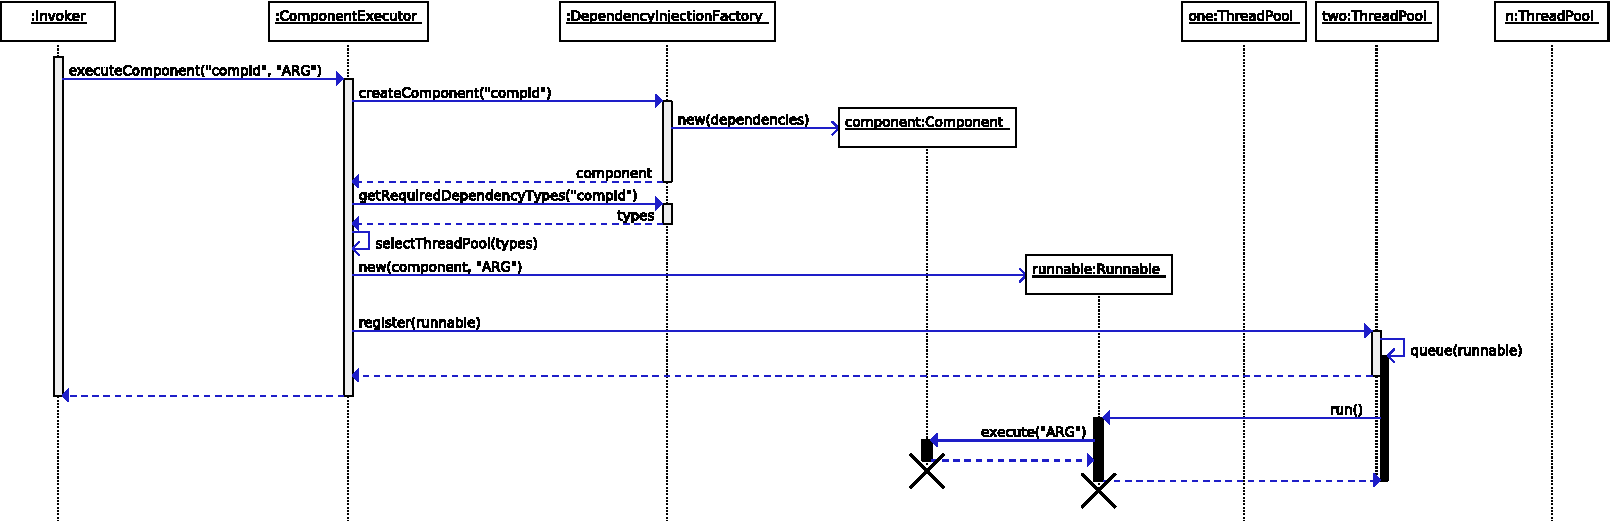
\includegraphics[width=6in]{ExecuteComponentSequenceDiagram}
\caption{Sequence diagram of invoking \texttt{executeTask(\ldots)} (Listing \ref{lst:TaskExecutionInterfaces}).  The \texttt{Task} is executed by one of the responsible thread pools configured by the developer.}
\label{fig:ExecuteComponentSequenceDiagram}
\end{figure}

The \texttt{getRequiredDependencyTypes(\ldots)} (Listing
\ref{lst:TaskExecutionInterfaces}) method provides the categorisation of the
\texttt{Task}.  As the arguments to the method are supplied to its wrapping
\texttt{Task} by \textsc{dependency injection}~\cite{ioc}, the
\texttt{getRequiredDependencyTypes(\ldots)} method uses the \textsc{dependency
injection} configuration\footnote{OfficeFloor uses qualification to distinguish
dependencies of the same type and returns a type object containing both class
and qualifier.  The thread pool matching incorporates the qualifier.} to
identify the required parameter types of the method within the \texttt{Task}
(\textsc{categorise task}).

The prioritisation tuning is achieved by use of responsible thread pools.  The
developer configures thread pools that are each responsible for \texttt{Task}s
with a particular type of dependency\footnote{Thread pools may be associated
with more than one dependency type.}.  To execute the \texttt{Task}, the
\texttt{Task} is matched by its dependency types to a thread pool responsible
for the dependency type\footnote{The \texttt{taskId} may also be used for very
fine grained responsibility.} (\textsc{responsible team}).  The
\texttt{execute()} method (Listing \ref{lst:TaskExecutionInterfaces}) is then
invoked by a thread from the matching thread pool to execute the \texttt{Task}.
This provides isolation of differing \texttt{Task}s to their respective
responsible thread pool for improved tuning of the server\footnote{The task
execution patterns are collectively identified as the software pattern
\textsc{thread injection}.  This is because the thread being chosen to execute
the method is undertaken in a similar way to the selection of dependencies by
the \textsc{dependency injection}~\cite{ioc} pattern.}.

For \texttt{Task}s not having dependencies (nor dependencies of any performance
significance), a default thread pool is used for their execution.  This ensures
all \texttt{Task}s are mapped to a thread pool.  It also means that thread pools
need only be configured for dependencies requiring isolation (i.e. all
\texttt{Task}s using the dependency are isolated to a particular thread pool for
execution).

To improve performance of runtime decisions the mapping of \texttt{Task} to
thread pool is cached.  As the dependencies for each \texttt{Task} is static, at
application start up time the \texttt{TaskExecutor} preprocess and caches the
mapping of \texttt{Task} to thread pools to reduce runtime decision overheads.
Conflicts arising from methods able to be mapped to multiple responsible thread
pools is resolved by ordering the thread pools and assigning \texttt{Task}s
based on first match.

To achieve further efficiencies the implementation of each thread pool is
specific to its responsible dependency type.  For example, the thread pool may
contain multiple threads for concurrent execution of \texttt{Task}s with threads
added or removed based on the load of \texttt{Task}s (\textsc{manage team sizes}),
a single thread for serial execution of \texttt{Task}s, or no threads;
executing \texttt{Task}s by borrowing the thread of control to reduce
thread-context switching (\textsc{do it yourself}).

The \texttt{cancel(\ldots)} method (Listing \ref{lst:TaskExecutionInterfaces})
enables the \texttt{TaskExecutor} to cancel the \texttt{Task}. The
\texttt{Task\-Executor} will cancel new \texttt{Task}s for a particular thread
pool when queuing the \texttt{Task} will result in exceeding a particular
threshold (\textsc{team too busy}).  Each thread pool has its own thresholds
particular to its responsible dependency type.  An example threshold is ensuring
the running average wait time for the thread pool's queue is below a certain
limit.  As \texttt{Task}s are mapped to particular thread pools, this ensures
only the appropriate \texttt{Task}s are cancelled.  Once cancelled the
\texttt{TaskExecutor} may discard the \texttt{Task}.  The implementation of the
\texttt{can\-cel(\ldots)} method is covered by the \textsc{escalation} pattern.


\subsubsection*{Consequences}

OfficeFloor provides improved performance tuning of applications operating in
complex enterprise environments that require integration with many downstream
systems (e.g. the reverse 10K problem~\cite{reverse-ten-k-problem} arising in
Service-Oriented Architectures).  Each downstream system's performance impacts
are isolated by assigning the downstream system's communication dependency its
own responsible thread pool.  This has requests that require a slow downstream
system to be queued on its responsible thread pool, allowing other requests
using different downstream systems to be serviced by other thread pools.

Furthermore, the isolation provided by using multiple thread pools enables
improved tuning of the server.  Tuning the thread pools (such as changing the
pool's thread nice values) allows the prioritising of threads and subsequently
prioritising groups of related methods.

For low load servers where a single thread pool is sufficient, having multiple
thread pools causes increased complexity for developer configuration.  While
OfficeFloor provides the flexibility to focus the tuning of isolated categories
of tasks by using responsible thread pools, it does place a burden on the
developer to understand thread related performance issues (e.g. costs related to
thread stack memory and thread-context switching) and the performance of the
dependencies (along with their related tasks).  In this case, a single
responsible thread pool is utilised for all tasks.  Then as conditions of the
application change requiring improved performance tuning, additional responsible
thread pools are introduced to enable the required performance tuning of the
application.

OfficeFloor loses its ability to effectively prioritise and cancel tasks if the
task dependencies are too similar.  For example, all request handling for
dynamic content by a web server is likely to reequire a database connection.
Whilst this will allow isolation of requests for static content, it will not
isolate requests for dynamic content serviced from cached data rather than
database data.  This is because the request handler (task) will depend on the
database connection to retrieve the data if the data is not cached.  As a
consequence, request handling will need to be segmented into smaller tasks. 
This is to reduce the occurrence of sets of common dependencies between tasks,
which results in grouping all of these tasks onto the same thread pool.  The task
collaboration patterns resolve this issue.


\subsubsection*{Related implementations}

JAWS~\cite{jaws} identified limitations in using a single concurrency model for
an application.  The JAWS framework enables multiple concurrency models to be
used by an application.  However, the concurrency models provided by the JAWS
framework are obtrusive to developer design requiring the developer to be
significantly involved with concurrency of the application.

The Staged Event-Driven Architecture (SEDA) \cite{seda} provides a similar
implementation to OfficeFloor without the use of the \textsc{categorise task}
pattern.  SEDA directly maps tasks to a stage and subsequently a thread pool.
However, the SEDA pipeline exhibits increased thread-context switching as a
result of hard stage boundaries, which prohibits threads to be borrowed (i.e.
not able to use \textsc{do it yourself}).

OfficeFloor can be considered a style of cohort scheduling \cite{cohort}, which
groups tasks with similar dependencies and infers from that similar
functionality.  However, OfficeFloor works at the application scheduling level
and allows the use of any operating system thread scheduling algorithms.

Capriccio~\cite{capriccio} utilises resource-aware scheduling of threads.  For
Capriccio to be resource-awareness, it uses information based on similar
techniques to \textsc{categorise task}.  This results in improved scheduling to
better release resources to undertake new tasks.  However, Capriccio is still
subject to thread starvation for slow tasks by using only a single thread pool.

Dependency capsules \cite{dependency-capsules} isolates the execution of tasks
by their dependencies to an alternate thread pool.  This is similar to
\textsc{responsible team}.  However, the dependency capsules require a
thread-context switch back to a main thread for executing tasks without
dependencies (i.e. can not use \textsc{do it yourself} to complete the request).

Hop~\cite{hop} enables developers to provide code to dynamically decide the
concurrency model for tasks at runtime.  Having the developer provide this code
involves the developer significantly with the concurrency issues of the
application.  Such issues are circumvented by the use of the performance tuning
provided by responsible thread pools.

Popular middleware servers use the \textsc{thread-per-request} pattern.
For example, popular web servers (Netcraft November 2012 survey) serve dynamic
web content by CGI/FastCGI with for example PHP scripts, Microsoft's
HTTP.sys/WAS, and JEE Servlets. These servers use the
\textsc{thread-per-request} pattern that is intuitive for developers to use.
However, these servers suffer from thread starvation within their single thread
pool by a slow task.  By isolating the slow task to its own responsible thread
pool, OfficeFloor overcomes a single slow task causing thread starvation across
all requests.

Modern event-based frameworks based on the \textsc{proactor} pattern, such as
Node.js~\cite{nodejs}, are enabling increased concurrency for applications.
However, the use of the \textsc{proactor} pattern forces interaction with
downstream systems to be non-blocking I/O.  OfficeFloor enables use of
non-blocking I/O via the \textsc{pick up task again} pattern.  Furthermore,
through responsible thread pools OfficeFloor enables prioritisation of blocking
I/O for more intuitive development.




\section{Patterns for collaboration of tasks}

The following patterns model the collaboration of methods on the way tasks
collaborate within an office.  The result of these patterns is that they
decouple the collaboration of methods.  The decoupling is necessary to overcome
the isolation limitations in the task execution patterns by tasks having too
similar dependencies.  Furthermore, these patterns provide the necessary
decoupling for the build process patterns of the next section.  The
implementation notes at the end provide details on how to implement the
patterns.


\subsection{\textsc{\textbf{hand-off}}}

\subsubsection*{Context} Within an office, teams hand-off to each other based on
the category of the next task.  For example, after financing a project the
finance team hand-off to the software development team to build the application.

Within software, method invocations tightly couple the thread of control and
prevent changing the thread of control in calling another method.

\subsubsection*{\textbf{Problem}} Enable changing the thread of control when calling
another method.

\subsubsection*{Forces} The calling of a method should still be intuitive for
the developer.

\subsubsection*{\textbf{Solution}}  Provide an interface as a parameter to the
method.  Each method of the interface asynchronously invokes a respective
handling method by registering the handling method for execution by a thread
pool.

\subsubsection*{Implementation note} A proxy implementation of the interface is
created by OfficeFloor and provided to the method by \textsc{dependency
injection}~\cite{ioc}.  The proxy implementation undertakes the asynchronous
invocation of the respective target method.

\subsubsection*{Consequences} The target method is asynchronously invoked by
another thread of control.  However, due to the asynchronous invocation no
return value is available from the invoked method.  Furthermore, each hand-off
incurs the cost of a thread-context switch.

\subsubsection*{Related Patterns} Is a sequence on \textsc{responsible team} to
hand-off methods to a responsible team.  This pattern has similarities to the
\textsc{mediator}~\cite{gof} pattern to keep methods from directly referring to
each other.  The \textsc{record information} pattern is used to provide return
values.



\subsection{\textsc{\textbf{escalation}}}

\subsubsection*{Context} Within an office, a person will escalate issues to
their manager rather than consult the person handing-off the task.  The person
handing-off the task is not in a position to handle issues with the task.  For
example, the finance team are not the correct team to escalate issues around
clarity of requirements when they hand-off funded development tasks to the
software development team.

Within software, the exception for a method (task) is thrown to the calling
method.  The caller is required to handle the exception or throw again to its
caller.

\subsubsection*{\textbf{Problem}} Escalate an exception to a handling method rather than
the calling method.

\subsubsection*{Forces} Method exceptions follow the method calls back to an
appropriate \texttt{try\ldots catch} block for handling the exception.

\subsubsection*{\textbf{Solution}} Intercept the exception and \textsc{hand-off} the
exception to a handling method.

\subsubsection*{Consequences} The caller does not deal with exceptions from
\textsc{hand-off} method invocations.  This means the caller will not be
aware of failures in its called methods.  However, it is unreasonable to have
the caller responsible for all downstream issues in the process flow.

\subsubsection*{Related Patterns} \textsc{hand-off} is used to enable the
exception to be handled by another method.  As \textsc{hand-off} is used, this
enables use of \textsc{record information} to make the calling method aware of
failures.



\subsection{\textsc{\textbf{define process flows}}}

\subsubsection*{Context} Within an office, a process is executed as a sequence
of tasks.  The actual sequence of tasks varies based on the outcome of the
current task being executed.  This is because for each outcome of the current
task there is an appropriate next task.  For example, before undertaking any
software enhancement the finance team checks if the client owes money.  If the
client owes money the software enhancement is not developed and the client is
sent a reminder for the outstanding money.

The process can be changed by altering the next task for an outcome of the
current task.  For the above example, on the client owing money the next task
can be altered to checking with the sales team.  The sales team can access the
client to determine whether the software enhancement should be undertaken to
keep a good relationship with the client.

Within software, the method directly specifies the next method (task) called.
The code requires altering in order to change the sequence that the methods are
executed.

\subsubsection*{\textbf{Problem}} Change the execution order of methods without
changing code.

\subsubsection*{Forces} Method invocation is tightly coupled at the code level.

\subsubsection*{\textbf{Solution}} Use \textsc{hand-off} and, via configuration,
map the hand-off interface method to a handling method.  Furthermore, provide a
hand-off upon completion of a method.  This completion hand-off is mapped to
execute a next method if no other hand-off is triggered (which includes
\textsc{escalation} hand-offs).

\subsubsection*{Consequences} Configuration maps the flow of methods rather than
being hard-coded within the method.  However, the resulting indirection will
make it difficult to follow the flow of the process.  Representing the
configuration graphically makes it easier and more intuitive to follow.  The
graphical configuration has tasks as nodes with hand-offs anchors on the task. 
The hand-off mapping configuration is directed lines from the hand-offs to their
respective handling task.

\subsubsection*{Related Patterns} \textsc{hand-off} enables the indirection to
use configuration to map the hand-off invocation to a handling method.




\subsection{\textsc{\textbf{do your work}}}

\subsubsection*{Context} Within an office, a team can be assigned to execute a
sequence of tasks.  Rather than passing the tasks around to different people in
the team, it is more efficient for one person to complete the sequence of tasks
without the overheads of hand-offs.

Within software, registering a method (task) for execution by a thread pool
(team) effectively has a different thread (person) execute the method.  Using a
different thread incurs thread-context switching that reduces the efficiency of
the application.

\subsubsection*{\textbf{Problem}} Avoid the thread-context switch when the hand-off
results in a method being executed by the same responsible thread pool.

\subsubsection*{Forces} The hand-off results in registering a method with a
thread pool for execution.  The next thread of the thread pool executes the
method.  Using the next thread will typically incur a thread-context switch to
execute the registered method.

\subsubsection*{\textbf{Solution}} Before registering the invoked method with its
responsible thread pool, check if the thread pool is the same responsible thread
pool of the current method.  If they are the same responsible thread pool
execute the invoked method synchronously (i.e. with the current method's thread
of control).

\subsubsection*{Consequences} Thread-context switching is reduced for sequential
methods of the same responsible thread pool\footnote{Combining \textsc{do your
work} with \textsc{do it yourself} provides the implicit thread of control.  The
implicit thread of control avoids thread-context switching in executing the
sequence of methods until an explicit thread (another responsible thread pool
containing threads) is required.}.  This also avoids queuing each task during
overload of the server that will result in \textsc{team too busy} cancelling
tasks for a greater number of existing processes.

\subsubsection*{Related Patterns} Is a sequence on \textsc{hand-off} to reduce
thread-context switching.



\subsection{\textsc{\textbf{task complete}}}

\subsubsection*{Context} Within an office, a person may need to know when the
tasks they have handed-off to other teams are complete.  For example, a sales
person will need to get back to the customer when the finance team has the
invoice ready.

Within software, the hand-off returns control to the calling method (task)
before the invoked method (task) is complete.  Therefore, the calling method is
uncertain as to whether the handed-off method is complete.

\subsubsection*{\textbf{Problem}} Know when the handed-off method is complete.

\subsubsection*{Forces} Methods invoked by hand-offs are asynchronously executed
by other threads.  There is no synchronous return from them to the calling
method to indicate when the handed-off method is complete.

\subsubsection*{\textbf{Solution}} Provide a Future from the hand-off invocation to
indicate when the handed-off method is complete\footnote{As the handed-off
method can invoke further hand-offs, the Future indicates when the resulting
tree of hand-offs is complete.}.  Furthermore, the checking of hand-off
completion is non-blocking so it does not tie up a calling thread.

\subsubsection*{Consequences} The Future provides a polling mechanism to check
when the handed-off method is complete.  Subsequently a thread is required to
poll the Future to determine completion.  However, when handing-off many methods
this enables distinguishing which are complete.

\subsubsection*{Related Patterns} The \textsc{pick up task again} pattern avoids
polling the Future.



\subsection{\textsc{\textbf{pick up task again}}}

\subsubsection*{Context} Within an office, notifying of when the handed-off tasks
are complete allows the calling team to get on with other work and return to the
task when the handed-off tasks are complete.  For example, the sales team can
seek out other customers and only get back in contact with a customer when the
financial team notifies them that an invoice is ready.

Within software, asynchronous invocations of methods (tasks) do not provide
notification back of the method's completion.

\subsubsection*{\textbf{Problem}} Notify the current method when a handed-off method is
completed.

\subsubsection*{Forces} The handed-off method is asynchronously invoked and there is
no synchronous return to indicate when it is complete.

\subsubsection*{\textbf{Solution}} Re-register the current method for execution again
when the handed-off method is complete\footnote{As the handed-off method may
invoke further hand-offs, the re-register only occurs when the resulting tree of
hand-offs is complete.}.

To simplify multi-threading issues the method is only re-registered once with
its responsible thread pool for re-execution.  There may be multiple hand-offs
that will result in multiple re-registering.  Having the method only registered
once for re-execution reduces multi-threading issues caused by concurrent
execution of the method by two or more threads.  After re-executing the method,
the method may again be registered for re-execution by further handed-off method
completions.

\subsubsection*{Consequences} There is no need to poll the Future of the
hand-off invocation.  Whilst waiting on many handed-off methods, the method may be
executed many times as each hand-off method completes.  The \textsc{task
complete} pattern is used as a guard condition to only execute the functionality
once all appropriate handed-off methods are complete.

\subsubsection*{Related Patterns} \textsc{task complete} is used to indicate
which handed-off methods are complete.  The \textsc{record information} pattern,
providing the state for the picked up again task, is similar to the
\textsc{asynchronous completion token}~\cite{posa} pattern.



\subsection{\textsc{\textbf{record information}}}

\subsubsection*{Context} Within an office, information is recorded for retrieval
and use in subsequent tasks.  For example, the sales team records the customer's
details that the finance team later use to raise an invoice for the customer.

Within software, methods (tasks) only use the arguments (information) supplied
from the calling method (task)\footnote{The method may also access implicit
references via its owning object.  However, this is to be avoided with the
\textsc{record information} pattern.}.

\subsubsection*{\textbf{Problem}} Enable the method to retrieve information from
previous methods other than its calling method.

\subsubsection*{Forces} Method invocation requires the caller to provide all
parameters to the invoked method.

\subsubsection*{\textbf{Solution}} Use \textsc{dependency injection}~\cite{ioc}
to inject cached dependencies as the arguments to the methods.

\subsubsection*{Consequences} As the cached dependencies provide state, they
enable all downstream methods in the process to retrieve the state.

Making the dependency state mutable allows upstream methods awareness of changes
in state when executed again via \textsc{pick up task again}.

\subsubsection*{Related Patterns} Is a sequence on \textsc{dependency
injection}~\cite{ioc} to cache dependencies and inject them as arguments to the
method.  The pattern has many similarities to \textsc{flyweight}~\cite{gof}.



\subsection{\textsc{\textbf{complete the form}}}

\subsubsection*{Context} Within an office, when handing-off to another team, the
receiving team will require certain information to carry on with the next task
in the process.  To ensure the receiving team has all the information necessary
for the particular hand-off, the handing-off team is required to complete a
form.  For example, for the financial team to raise a software defect, the
software development team requires the financial team to fill in a ticket (form)
with the details regarding the defect.

Within software, the method (task) defines many parameters (forms) that must be
supplied.  However, the hand-off invocation requires the parameters (forms) to
be standardised for a consistent hand-off interface.

\subsubsection*{\textbf{Problem}} Pass data to the handling method when the hand-off has
a standard interface.

\subsubsection*{Forces} The handling method invoked by the hand-off retrieves
its data via \textsc{record information} (cached dependencies).

\subsubsection*{\textbf{Solution}} Allow a single argument to be passed with the
hand-off that encapsulates the data to be passed.  For multiple arguments they
are to be encapsulated into a single object (argument).  The argument is made
available to the handling method as a dependency via \textsc{record
information}.

\subsubsection*{Consequences} The handling method need not differentiate between
the hand-off passed argument and the dependencies obtained from \textsc{record
information}.

Providing an argument does restrict the \textsc{define process flows}
configuration, as the invoked method's parameter type must match the handed-off
argument type.  Using an adapter task (as per the \textsc{adapter}
pattern~\cite{gof}) in between the tasks removes this restriction.  The adapter
task transforms the hand-off argument to the required parameter type.

\subsubsection*{Related Patterns} Is a sequence on \textsc{hand-off} and
\textsc{record information} to enable the caller to pass data with the hand-off.



\subsection{\textsc{\textbf{contact us}}}

\subsubsection*{Context} Within an office, it is inefficient for all customers
to have to go through the front desk to contact a particular team.  Hence, teams
within the office provide contact details to enable direct engagement by people
external to the office.

Within software, references to methods (tasks) are only available within the
application (office).

\subsubsection*{\textbf{Problem}} Handing-off the first method (task) when not
provided a hand-off interface, as the caller is outside the application
(office).

\subsubsection*{Forces} The interface to invoke a hand-off is only provided to
methods being executed within a task of the application.

\subsubsection*{\textbf{Solution}} Provide a unique address (e.g. URL) that directly maps
to the initial method.  Sending a request to this address invokes the hand-off
for the first method.

\subsubsection*{Consequences} Methods are called from outside the application. 
Responses are achieved by \textsc{record information} providing the data for a
response\footnote{\textsc{record information} also provides access to the client
connection to send the response.}.

\subsubsection*{Related Patterns} Is a sequence on \textsc{hand-off} to enable
external applications to hand-off to this application.



\subsection{\textbf{Implementation notes for the task collaboration patterns}}

\subsubsection*{Background}

Both the \textsc{thread-per-request} pattern \cite{thread-per-request} (basis of
many mainstream middleware designs) and the \textsc{proactor} pattern
\cite{proactor} (basis of event-driven middleware designs) impose tight coupling
on the collaboration of tasks (objects wrapping the execution of a method).  The
\textsc{thread-per-request} pattern enables invoking tasks by synchronous
methods, which is intuitive for developers \cite{proactor}.  In contrast, the
\textsc{proactor} pattern enables asynchronous invocation of a constructed task
by registering it for execution by another thread of control (allowing the
execution of tasks concurrently).  Both patterns tightly couple the
collaboration of tasks, since the \textsc{thread-per-request} pattern must have
the caller provide the thread of control and the \textsc{proactor} pattern must
have the caller construct the invoked task.

The \textsc{thread-per-request} pattern and \textsc{proactor} pattern further
tightly couple collaboration of tasks by the caller being required to handle
exceptions.  The caller may not be appropriately responsible to handle a
resulting exception and this should be handled by another task.


\subsubsection*{Implementation}

The task collaboration implementation builds on the task execution
implementation.  On executing a \texttt{Task} (object wrapping the method) the
\texttt{Task} is provided a \texttt{TaskContext} (Listing
\ref{lst:TaskCollaborationInterfaces}).

\lstset{caption=Task collaboration pattern interfaces.}
\begin{lstlisting}[float,label=lst:TaskCollaborationInterfaces]
    interface Task {
        void execute(TaskContext context);
        String[] getHandOffIds();
        String[] getStateIds();
    }

    interface TaskExecutor {
        Future executeTask( String taskId 
                          , Object parameter
                          , DependencyContext context);
    }

    interface TaskContextFactory {
        TaskContext createTaskContext( String taskId
                                     , Object parameter
                                     , DependencyContext context);
    }

    interface TaskContext {
        Object getState(String stateId);
        Future doHandOff(String handOffId, Object parameter);
        void handleException(Exception exception);
        void setComplete(boolean isComplete);
    }

    interface DependencyInjectionFactory {
        Type[] getRequiredDependencyTypes(String dependencyId);
        DependencyContext createDependencyContext();
    }
    
    interface DependencyContext {
        Object getDependency(String dependencyId);
    }

    interface Office {
        Future doProcess( String initialTaskId
                        , Object initialTaskParameter);
    }
\end{lstlisting}

\begin{figure}[!t]
\centering
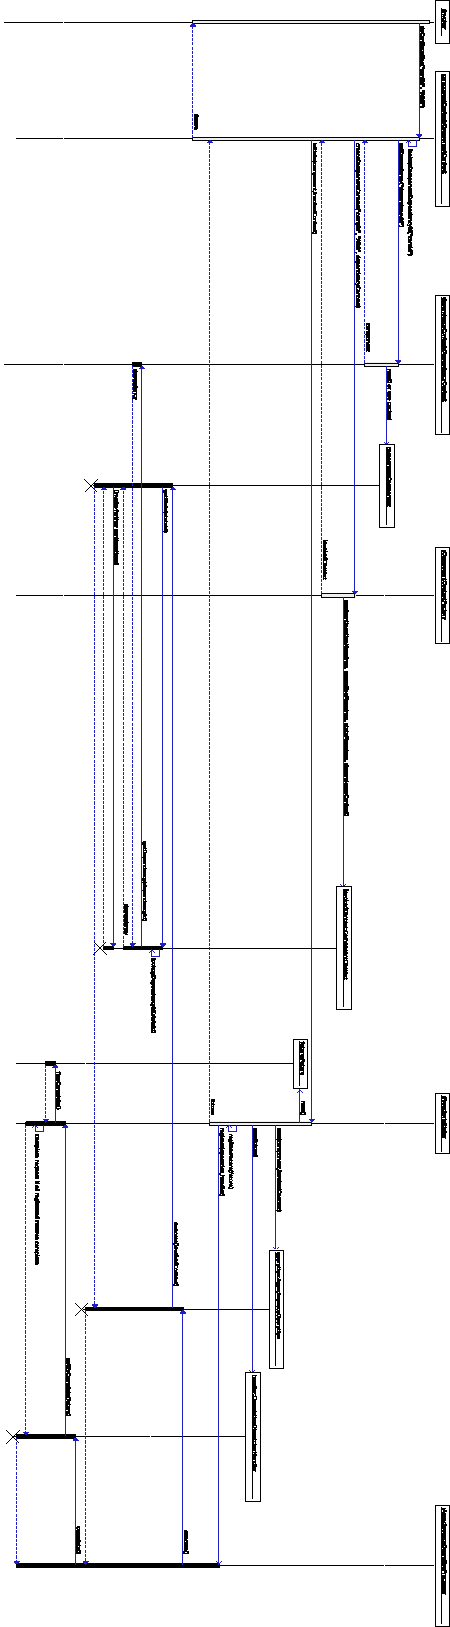
\includegraphics[height=7.4in]{DoContinuationSequenceDiagram}
\caption{Sequence diagram of invoking \texttt{doHandOff(\ldots)}.}
\label{fig:DoContinuationSequenceDiagram}
\end{figure}

For the method within the \texttt{Task} to collaborate with other methods it
defines a hand-off interface (Listing \ref{lst:Example_Method_Task} provides an
example hand-off interface).  The \texttt{Task} wrapping the method creates a
proxy implementation of the hand-off interface.  The proxy implementation wraps
the \texttt{TaskContext} (Listing \ref{lst:TaskCollaborationInterfaces}) and
invokes \texttt{doHandOff(\ldots)} with the invoked interface method name as the
\texttt{handOffId} (\textsc{hand-off}).  As the \texttt{handOffId}s are static
for each \texttt{Task}, developer configuration provides the hand-off mapping to
the respective handling \texttt{Task}\footnote{OfficeFloor enhances the
\texttt{getHandOffIds()} method to also return the argument types that the
\texttt{Task} will provide on each of the hand-offs.  OfficeFloor also enhances
\texttt{getStateIds()} to provide the expected type the \texttt{Task} requires
for each \texttt{stateId}. Providing this type information enables the hand-off
argument to be type validated against the handling \texttt{Task}'s required
parameter type.  This reduces runtime errors by providing type validation of the
\textsc{define process flows} configuration.} (\textsc{define process flows}). 
Figure \ref{fig:DoContinuationSequenceDiagram} provides a sequence diagram of
invoking a \texttt{Task} via the \texttt{doHandOff(\ldots)} method.

The \texttt{TaskContextFactory} (Listing \ref{lst:TaskCollaborationInterfaces})
constructs the \texttt{TaskContext}.  The \texttt{TaskContextFactory} centrally
manages the hand-off (\texttt{handOffId}) mapping to target \texttt{Task}
(\texttt{taskId}).

To avoid relying on \texttt{Task}s to define hand-offs, each \texttt{Task} has
an implicit hand-off.  The implicit hand-off is triggered on completion of the
\texttt{Task} should no other hand-offs be invoked.  This enables configuring a
sequence of \texttt{Task}s as sequential steps of a process (\textsc{define
process flows}).

The hand-off triggers the \texttt{TaskExecutor} to register a \texttt{Task} with
its responsible thread pool for asynchronous execution.  A \texttt{Future} is
returned from this registration to indicate when the handed-off \texttt{Task} is
completed (\textsc{task complete}).  The \texttt{TaskExecutor} is also notified
of completion of the \texttt{Task}.  This enables the \texttt{TaskExecutor} to
re-register any \texttt{Task}s waiting on the \texttt{Future} (\textsc{pick up
task again}).  \texttt{Task}s flag that they need re-registering by calling
\texttt{setComplete(\ldots)} (Listing \ref{lst:TaskCollaborationInterfaces})
indicating the \texttt{Task} is not complete.

A \texttt{TaskExecutor} instance is created per process instance.  This enables
the life-cycle of \texttt{Task}s to be aligned with the process\footnote{The
\texttt{TaskExecutor} implementation within OfficeFloor also models the software
concept of a thread.  The hand-off configuration mapping has an attribute
indicating whether the hand-off spawns a thread (new \texttt{TaskExecutor}).}.
It also enables the \texttt{TaskExecutor} to register \texttt{Task}s that are
executed on completion of the process.  For example, registering a \texttt{Task}
to send the response at the end of the process.

Each \texttt{Task} is constructed via the \textsc{dependency injection} pattern
\cite{ioc}.  The \texttt{Dependency\-InjectionFactory} (Listing
\ref{lst:TaskCollaborationInterfaces}) centrally manages the dependency
configuration for all \texttt{Task}s.  To enable sharing state between
\texttt{Task}s, the \texttt{Dependency\-InjectionFactory} creates a
\texttt{Depend\-ency\-Context} that caches the dependency instances for the
\texttt{Task}s.  As the dependency instances are re-used across \texttt{Task}s,
this shares state between the \texttt{Task}s (\textsc{record information}).
Furthermore, as the \texttt{Dependency\-Context} manages the life-cycle of
dependencies, it is aligned to the \texttt{TaskExecutor} life-cycle.
This enables both the dependencies of the \texttt{Task}s and the \texttt{Task}s
themselves to be specific to the instance of the process.

The \texttt{doHandOff(\ldots)} method does allow one argument to be passed to
the invoked \texttt{Task} (\textsc{complete the form}).  This is for more
intuitive development by passed state with the hand-off.  If multiple arguments
are required they are encapsulated into an object for passing.  To maintain
loose coupling the invoked \texttt{Task} obtains the argument as state (i.e.
\texttt{getState(\ldots)} method in listing
\ref{lst:TaskCollaborationInterfaces}).  This is so the invoked \texttt{Task}
need not differentiate between dependencies and the passed argument
(\textsc{record information}).  The invoked \texttt{Task} may also ignore the
handed-off argument should it not depend on it.

The hand-off will borrow the thread of control of the calling \texttt{Task} if
it results in being executed by the same thread pool.  Rather than dispatching
the \texttt{Task} back to the same thread pool, the \texttt{TaskExecutor}
borrows the thread to execute the next method (\textsc{do your work}). This
avoids the overhead of a thread-context switch.

Exceptions from the methods are handled by being mapped to a \texttt{handOffId}.
The \texttt{Task} invokes \texttt{handle\-Excep\-tion(\ldots)} with the
exception from the method.  The \texttt{handleException(\ldots)} method is
implemented by mapping the exception type to a \texttt{handOffId} and invoking
the \texttt{doHandOff(\ldots)} method with the exception as the argument
(\textsc{escalation}).  The developer configures hand-offs for specific
exception types (\textsc{define process flows}).  The developer will also
configure ''catch all'' hand-offs to handle exceptions from any \texttt{Task} to
ensure all exceptions are handled (e.g. handling of the runtime non-checked
exceptions).

Integrating with code not contained in \texttt{Task}s does not allow access to
the \texttt{TaskContext}.  The \texttt{Office} (Listing
\ref{lst:TaskCollaborationInterfaces}) provides an interface that allows code
not contained in a \texttt{Task} to trigger the hand-off for the first
\texttt{Task}.  The returned \texttt{Future} indicates when all \texttt{Task}s
of the process are complete.  To retrieve results the \texttt{parameter} is used
as a visitor (\textsc{visitor} pattern \cite{gof}) and loaded with results by
the invoked \texttt{Task}s (\textsc{record information}).  The
\texttt{initialTaskId} is mapped to a unique URL for external triggering of the
process (\textsc{contact us}).



\subsubsection*{Example}

Listing \ref{lst:Example_Method_Task} shows an example method for retrieving
data from a cache.  The \texttt{Task} for the \texttt{retrieve\-Data(\ldots)}
method will:
\begin{enumerate}
  \item Obtain an instance of the \texttt{CacheOperation} via the \texttt{getState(\ldots)} method.
  \item Obtain both the \texttt{key}\footnote{\texttt{key} is a hand-off argument from the previous \texttt{Task}.} and \texttt{cache} again via the \texttt{getState(\ldots)} method.
  \item Instantiate a proxy implementation of the \texttt{CacheHandOffs} interface that wraps the \texttt{TaskContext}.  The proxy implements the \texttt{cacheMiss(\ldots)} method by invoking \texttt{doHandOff(``cacheMiss'',key)}. 
  \item Reflectively invoke the \texttt{retrieveData(\ldots)} method with the above arguments.
\end{enumerate}

\lstset{caption=Example developer code of a method within a task for retrieving data from a cache.  \texttt{CacheHandOffs} is the hand-off interface for the \texttt{retrieveData(\ldots)} method.}
\begin{lstlisting}[float,label=lst:Example_Method_Task]
  class CacheOperation {
    public Data retrieveData(String key, Cache cache
                            , CacheHandOffs handOffs
                            ) throws IOException {
        Data data = cache.get(key);
        if (data == null) {
            handOffs.cacheMiss(key);
            return null; // finish task
        }
        return data;
    }
  }

  interface CacheHandOffs {
    Future cacheMiss(String key);
  }
\end{lstlisting}

Hand-offs from the \texttt{retrieveData(\ldots)} method are:
\begin{itemize}
  \item \texttt{cacheMiss(\ldots)} which is mapped to a \texttt{Task} to retrieve data from the database.
  \item Implicit hand-off which is mapped to the next \texttt{Task} in the process\footnote{The return value from the method is used as the implicit hand-off argument.}.
  \item \texttt{IOException} which is mapped to a \texttt{Task} providing an error response.  It may also be mapped to a \texttt{Task} to retrieve the data from a database to attempt to continue the process.
\end{itemize}


\subsubsection*{Consequences}

The task collaboration patterns enable decomposing the functionality into
smaller tasks.  As methods within the \texttt{task}s collaborate through
\textsc{hand-off}, the methods are decoupled from each other.  Furthermore, the
decoupling through \textsc{record information} enables the methods to only
require a subset of the dependencies of the process.  Requiring only a subset of
the dependencies removes the task execution limitation of too many similar
dependencies causing all \texttt{task}s to be executed by the same thread pool.

The mapping of hand-off (\texttt{handOffId}) to \texttt{Task} (\texttt{taskId})
is contained within configuration.  This enables changing the invoked method
(\texttt{Task}) without changing the code of the methods.  Changing the handling
\texttt{Task} enables re-ordering the chained sequence of \texttt{Task}s that
are executed for the process.  This removes the invocation coupling of the
\textsc{proactor} pattern.  Furthermore, each \texttt{Task} is executed by a
thread from its responsible thread pool (i.e. potentially different thread). 
This removes the thread of control constraint imposed by the
\textsc{thread-per-request} pattern.

Understanding the collaboration of \texttt{Task}s would become difficult due to
the indirection involved.  However, the \textsc{define process flows}
configuration reduce this difficulty by providing means for graphical tools to
manage the configuration.  The tools graphically represent the \texttt{Task}s as
nodes and the hand-off mappings as directed lines between these nodes.  Due to
the similarity of this configuration with Service Orchestration this graphical
configuration is identified as Task Orchestration.

Furthermore, as the \texttt{Task}s are executed by different threads of control,
the stack trace automatically provided by the \textsc{thread-per-request}
pattern no longer reflects the call hierarchy.  This can make it difficult to
debug issues.  However, the \texttt{TaskExecutor} records the tree of
\texttt{Task}s invoked so that the tree can be traversed back to the root.
Hence, this identifies the sequence of hand-offs to the \texttt{Task} throwing
the exception.  The whole tree can also be reported to aid the developer in
debugging the cause of the issue.

Functions can also be used in place of methods.  When implementing
\texttt{Task}s with functions, the functions will not be pure.  As state is
shared between \texttt{Task}s by mutable state within dependencies, functions
will need to cause side effects (mutate state) to share state with other
\texttt{Task}s.



\subsubsection*{Related implementations}

OfficeFloor can be considered a form of continuation-passing style
\cite{continuations}.  The hand-off is similar to a continuation, as it is a
``goto'' for executing another \texttt{Task} with a different thread
(stack)\footnote{The task collaboration patterns are identified collectively as
the software pattern \textsc{continuation injection}.  The name comes from the
hand-offs (continuations) being injected into methods in a similar way to the
dependencies of the \textsc{dependency injection}~\cite{ioc} pattern.}.  The
benefit of providing hand-offs through a \texttt{TaskContext} is that the
\texttt{Task} is free to depend on as many hand-offs as necessary, and not what
the caller provides.  It also means that as the application evolves the
\texttt{Task} encapsulates potential changes requiring different hand-offs.  The
indirection allows managing these changes as configuration changes rather than
code changes.

The combined \textsc{do your work} pattern and \textsc{do it yourself} pattern
of OfficeFloor has similarities to a monadic thread \cite{monadic-thread}.  The
\texttt{Task}s can be considered nodes in the lazy trace of the monadic thread. 
The lazy trace ends when another thread of control is required.  The advantage of
OfficeFloor\footnote{Beyond Task Orchestration being easier for the developer to
understand than monad programming.} is that the \textsc{responsible team}
pattern allows the execution of blocking I/O nodes (\texttt{Task}s) to be
prioritised.  Monadic threads can not prioritise blocking I/O nodes as they know
little about them and subsequently execute them within a single thread pool.

OfficeFloor can be considered an implementation of the Actor Model \cite{actors}
as it adheres to the principles of the Actor Model.  The \texttt{Task} is the
actor.  The asynchronous communication between \texttt{Task}s decouples the
hand-off argument (message) from the sending \texttt{Task} (actor).  The
\texttt{taskId} provides an address for a \texttt{Task} (actor).  The provided
\texttt{handOffId}s restricts the \texttt{Task}s (actors) that may be used.




\section{Patterns for building processes}

The following patterns compose methods into composite functionality in a similar
way to processes within an office being constructed from tasks.  These patterns
address the second software problem addressed by this paper - creation of a
technical framework that enables delivery of working code earlier and
continuously.  The implementation notes at the end provide details on how to
implement the patterns.


\subsection{\textsc{\textbf{task defines itself}}}

\subsubsection*{Context} Within an office, the nature of the task will determine
which inputs are relevant and the stages at which delegation to other tasks is
necessary.  Unless the task is simple, providing the person executing the task a
fixed set of inputs and a fixed set of hand-offs will result in the task being
unsuccessful.  To be successful the person executing the task will seek out the
required inputs and other people necessary to complete the task.

Furthermore, when conditions change the task may require new inputs and new
hand-offs.  Introducing these new inputs and hand-offs should be encapsulated by
the task and not significantly impact its containing process.

Within software, the method signature is fixed by the caller of the method
(calling task) and not the implementation of the method (i.e. not the task
itself).  The caller provides all the arguments (inputs) and all the
object references (hand-offs) to the invoked method along with the thread of
control (person) to execute the invoked method.

\subsubsection*{\textbf{Problem}} Let the method implementation define the method
signature and continue to enable the caller to invoke the method as the method
signature changes.

\subsubsection*{Forces} The caller of a method:
\begin{itemize}
  \item identifies the method by name,
  \item provides all arguments to the method,
  \item handles all exceptions from the method,
  \item executes the method with its thread of control.
\end{itemize}

\subsubsection*{\textbf{Solution}} Use \textsc{hand-off} and \textsc{complete the form}
to decouple the caller from the method signature.  To enable the method
implementation to define the method signature, use:
\begin{itemize}
  \item \textsc{define process flows} to have the method define its name (\texttt{taskId}),
  \item \textsc{record information} to provide the arguments,
  \item \textsc{hand-off} to specify collaboration with other methods,
  \item \textsc{escalation} to handle exceptions, and
  \item \textsc{categorise task} (via \textsc{responsible team}) to specify the thread of control.    
\end{itemize}

\subsubsection*{Consequences} The caller is no longer coupled to the method
signature.  This allows the method signature to change without impacting the
caller.

The Task Orchestration visual representation of \textsc{define process flows} is
necessary to understand the flow of the application code, as the call
hierarchies can no longer be determined by method signatures.



\subsection{\textsc{\textbf{process defines itself}}}

\subsubsection*{Context} Within an office, the process is constructed from
tasks.  The process encapsulates the collaboration of the tasks and becomes the
sum of the functions within the tasks.  However, as the tasks define themselves,
the process is also subject to the necessities of its containing tasks.  The
process, therefore, also becomes the sum of all the dependencies and hand-offs
of its containing tasks.

Furthermore, determining whether the functions should be encapsulated in a task
or whether it should be a process involving multiple tasks executed by differing
responsible teams is typically not known at first.  Initially this may be
determined correctly.  However, over time conditions may change causing a
task to become more complex requiring it to be transformed into a process
involving many tasks and many responsible teams (or vice-versa being transformed
from a complex process to a simpler task).

Triggering a process within in an office is no different to triggering a task.
Like the task, the caller of the process is decoupled from the process.
\textsc{complete the form} is undertaken and a \textsc{hand-off} occurs to the
first task of the process.  Similar to the task, the process will
\textsc{escalate} issues and will \textsc{hand-off} to other processes/tasks as
necessary.

Therefore, within an office the process defines itself to achieve its
requirements\footnote{Process defining itself is similar to the process owner in
the business defining the process to meet the requirements.}.  The process is
also interchangeable with a task depending on the required complexity.

Within software, objects and their methods (tasks) are encapsulated into a
component (process).  Like the method signature, the interface to the component
is controlled by the caller.  Therefore, the component does not have control
over defining itself.

\subsubsection*{\textbf{Problem}} Enable each process (composition of tasks,
i.e. component) to define itself.  Furthermore, in defining itself the process
must have a similar interface to a task in order to be interchangeable with a
task.

\subsubsection*{Forces} Adding new tasks to a process is similar to adding new
functionality to a component.  Adding new functionality involves:
\begin{itemize}
  \item new dependencies that need to be referenced from the functionality,
  \item new exceptions that may occur from the functionality, and
  \item a potentially different threading model to efficiently undertake the functionality. 
\end{itemize}

\subsubsection*{\textbf{Solution}} Represent the process as a task in the
\textsc{define process flows}.  The process is given its own identifier that
maps to the initial task of the process\footnote{The process may expose multiple
\texttt{taskId}s to enable starting at different \texttt{Task}s within it.}.
All hand-offs not mapped to a task within the process become the set of
hand-offs for the process (this includes \textsc{escalation}).  All dependencies
of the contained tasks (from \textsc{record information}) becomes the set of
dependencies for the process.

To reduce the set of dependencies for the interface of the process, the same
dependency used by many of its contained tasks is represented as single
dependency of the process.

Also, to reduce the hand-offs for the interface of the process, hand-offs from
multiple contained tasks are mapped to a single hand-off exposed from the
process.

\subsubsection*{Consequences} As the process is interchangeable with a task,
composite processes are built from other processes.  The interface of a
composite process is created in the same way as if it contained tasks.

Having composite processes constructed from other composite processes requires
the graphical representation of the \textsc{define process flows} pattern (Task
Orchestration).  This is necessary for the developer to understand the flows
within the application, as adding composite processes is further indirection
that requires visual representation to comprehend.

The \textsc{categorise task} pattern of each contained task within the process
(and composite processes) is still followed.  As the process is constructed from
only tasks, the process focuses only on functionality and allows all its tasks
to be executed by their respective \textsc{responsible team} pattern.
Therefore, if the responsible thread pools are changed for the application the
execution of the tasks within the processes follow the new threading model
without requiring code nor configuration changes\footnote{Changing the
responsible thread pools follows the analogy of changing the functional (teams)
departments within a business.  The functional departmentalisation to execute
the tasks of the processes are changed while the sequence of tasks for the
process is not changed.}.  This enables the threading model of the application
to be tuned to the hardware on which it is running (e.g. single thread pool for a low
powered single CPU device or multiple specialised thread pools for
high-performance multi-core hardware\footnote{Using increasingly better hardware
follows the analogy of growing the workforce of a business.  The business starts
out only as a small number of people doing many categories of tasks to becoming
a large number of people doing very specific categories of tasks.}).



\subsection{\textsc{\textbf{automate only where appropriate}}}

\subsubsection*{Context} Within an office, automation of a process requires
maturing the process \cite{process-maturity-global,bpm-tools}.  Maturing a
process for automation requires the process to be identified and defined. 
Defining the process requires specifying the sequence of tasks, the dependencies
necessary for those tasks and catering to all the exceptions that may occur from
those tasks.

Within software, designing a system top-down requires all business processes to
be of a higher maturity.  Higher maturity processes provide the necessary
definitions (requirements) of what the software must automate.  Without these
requirements the software designers are unclear on what to automate.
Furthermore, each process implementation must fit within the top-down design of
the software system.  Without understanding each process it can not be
determined whether the system's design adequately caters to each process.
Therefore, to gain this understanding a higher maturity of the processes is
required due to the need to identify and define each process.

\subsubsection*{\textbf{Problem}} Design applications bottom-up so that
functionality (processes) may be incrementally added.

\subsubsection*{Forces} The method puts the control at the higher-level layers
of the application design.  The higher-level layer caller tightly couples the
method signature that the lower-level layers must implement.  The lower-level
layers can not change the method signature without refactoring the higher-level
layers due to this tight coupling.  This forces a top-down approach to designing
the application.

\subsubsection*{\textbf{Solution}} Use \textsc{task defines itself} to only use
proven tasks.  Then incrementally build only the identified and defined
processes through \textsc{process defines itself}.

\subsubsection*{Consequences} Using \textsc{task defines itself} and
\textsc{process defines itself} enables the design of the application to
automate only the mature processes within the business.  The less mature
processes are left undefined until they mature in the business.  Once the
process subsequently becomes mature enough it is added to the application.

This approach to designing applications aligns both to the maturing of business
processes and Agile development.  Agile focuses on early and continuous delivery
of working software \cite{agile-manifesto}.  Through \textsc{process defines
itself}, processes are built without requiring all other processes to be
identified and defined.  Therefore, the mature processes that provide value back
to the business are able to be built earlier.  Then as the other processes
mature, they are incrementally built into the application for continuous
delivery of new functionality.


\subsection{\textbf{Implementation notes for the process building patterns}}

\subsubsection*{Background}

Applications built with \textsc{layers} typically impose a top-down approach to
design.  ``The \textsc{layers} require and provide \textsc{explicit interfaces}
from and to each other, in a top-down manner, from the higher to the lower
\textsc{layers}'' \cite[p. 11]{ioc}.  The higher-level layer components (object
that wraps a method) define the variation points that are ``predefined points in
the control and data flow which allow for modifying and extending a component's
behaviour'' \cite[p. 5]{ioc}.  A top-down approach is required, as the
higher-level layer components control what variation points may be implemented
by the lower-level layer components.

The components need to be composed within an architecture that is dictated by
the framework.  The framework ``will define the overall structure, its
partitioning into \ldots [components], the key responsibilities thereof, how the
\ldots [components] collaborate, and the thread of control'' \cite[p. 26]{gof}.
Using the components within a framework, therefore, identifies the following
requirements of a component's \textsc{explicit interface}:
\begin{itemize}
  \item components must have a key responsibility;
  \item components must be able to collaborate with other components; and
  \item components require a thread of control.
\end{itemize}

The collaboration of components can further be defined as the following
requirements:
\begin{itemize}
  \item components must be able to invoke other components;
  \item components must be able to share state; and
  \item exceptions from components need to be handled.
\end{itemize}

Within frameworks, the method signature is the interface between components.
``The set of all [method] signatures defined by an object \ldots characterizes
the complete set of requests that can be sent to the object'' \cite[p. 13]{gof}.
As frameworks are composed of objects, the method signature defines the
interface between objects and subsequently components.

The method signature meets the requirements as it:
\begin{itemize}
  \item has a key responsibility identified by its name;
  \item may invoke other methods;
  \item shares state with other methods by arguments and return values;
  \item provides declaration of exceptions for handling; and
  \item can be executed by the thread of control.
\end{itemize}

The method interface is, however, subject to tight coupling.  The tight
coupling occurs from the calling higher-level layer component having to:
\begin{itemize}
  \item define the method name;
  \item provide the necessary arguments;
  \item possibly use the return value;
  \item handle potential exceptions; and
  \item provide the thread of control to execute the method.
\end{itemize}

This tight coupling imposed by the method results in the hierarchical
\textsc{layers} architecture where variation points (\textsc{explicit
interfaces}) are controlled by the higher-level layers.  The higher-level layer
component provides a \textsc{template method} \cite{gof} which is the variation
point that lower-level layer components may extend.

Within a \textsc{layers} architecture having variation points defined by
\textsc{template method}s requires refactoring of the \textsc{template method}
to increase the variability of the lower-level layer components.  Increasing the
variability ``requires adapting the \textsc{explicit interfaces} between the
\textsc{layers} to stipulate the types of variation parameters'' \cite[p.
5]{ioc} to allow control over the lower-level layers by the higher-level layers.

Instead of attempting to define variation points at the higher-level layers to
cover all possible variations of the lower-level layers, control should be
inverted and given to the lower-level layers to define the variation points.
However, given that the \textsc{template method} imposes a top-down control over
variation points, another form of \textsc{explicit interface} is necessary for
lower-level layer components to provide bottom-up control over defining
variation points for the application.



\subsubsection*{Implementation}

\textsc{record information} enables the lower-level layer component to specify
the state (objects) it requires.  The lower-level layer component specifies its
required state (objects) via \texttt{stateId}s.  As the lower-level layer
retrieves its state via \textsc{record information}, the invoking higher-level
layer components need only provide the single optionally used argument
(\textsc{complete the form}).  This allows the lower-level layer component to
specify as many dependencies as is necessary.  Therefore, it gives the
lower-level layer component control over what state (dependencies) it
may depend on.

\textsc{categorise task} enables the lower-level layer component to specify its
thread of control.  With the lower-level layer component having control over
specifying its required dependency types, the lower-level layer component may
specify additional dependencies to control which responsible thread pool will be
used to execute it.

\textsc{hand-off} enables the lower-level layer component to specify its
required collaboration by \texttt{handOffId}s.  The mapping of
\texttt{handOffId} to \texttt{taskId} (\textsc{define process flows}) enables
configuring of the higher-level layer components for handling each required
hand-off by the lower-level layer component.  As the higher level-layer
component does not need to provide references to these handling components on
calling the lower-level layer component, the lower-level layer component may
specify as many hand-offs as are necessary for its required collaboration
variation points.  This gives the lower-level layer component control over its
collaboration variation points.

Exceptions from components are handled by \textsc{escalation}.  The exception is
mapped to a \texttt{handOffId} and subsequently mapped to a handling component. 
As the invoking higher-level layer component is decoupled from having to handle
the exceptions, the lower-level layer component is free to throw as many
exceptions as is warranted.  This gives the lower-level layer component control
over its exceptions.

Using the office patterns provides the necessary inversion of control over
variation points, as the lower-level layer component controls:
\begin{itemize}
  \item its name (\texttt{taskId}) which is decoupled from the invoking higher-level layer component invocation (\texttt{handOffId}) by \textsc{define process flows};
  \item which invocations (\texttt{handOffId}s) are necessary via \textsc{hand-off};
  \item what state (\texttt{stateId}s) is required by \textsc{record information};
  \item the types of exceptions that may be thrown by \textsc{escalation}; and
  \item the thread of control by \textsc{categorise task} specifying the \textsc{responsible team}.
\end{itemize}

Therefore, the \texttt{Task} interface (Listing
\ref{lst:TaskCollaborationInterfaces}) is an \textsc{explicit interface} for a
component that provides inversion of control for the method signature.
Rather than the caller defining the method signature, the implementation of the
method controls the defining of the method signature (\textsc{task defines
itself}).

To manage the complexity of the application's functionality, OfficeFloor
modularises the \textsc{define process flows} configuration (Task Orchestration)
into sections.  Each section contains hand-off mapping configuration between
\texttt{Task}s and other contained sections (\textsc{process defines itself}).
The lower-level layer sections configure the \texttt{Task}s together.  The
higher-level layer sections configure these lower-level layer sections together.
As sections are configured from other existing sections, it creates a bottom-up
approach to building the application\footnote{OfficeFloor configures the
top-level sections within an office.  The office configuration enables weaving
further \texttt{Task}s as aspects into the contained sections (identified as the
\textsc{administration} pattern).  The office configuration also provides
additional management over dependencies, such as demarcating transactions
(identified as the \textsc{governance} pattern). OfficeFloor then configures
these offices onto the office floor where the dependencies and responsible
thread pools are configured.  The office building (agent running on each server)
hosts each office floor as a separate operating system process.  These patterns
will be included in the future work of usage patterns to build applications with
OfficeFloor.}.

Furthermore, the top-down approach to designing an application requires
understanding the entire scope of the application requirements.  Without
understanding all the complexities, the design may not adequately meet the
business needs and require significant refactoring to align with the business
needs.  OfficeFloor enables building only the mature processes bottom-up
(\textsc{automate only where appropriate}).  This removes the need to understand
all complexities as only understanding of the scope of each process to automate
is required.


\subsubsection*{Consequences}

Using \textsc{automate only where necessary} enables bottom-up control over the
design of the application.  As the variation points of the application are
controlled by the \texttt{Task}s (\textsc{task defines itself}), developers
start by building the \texttt{Task}s first.  As the \texttt{Task}s are less
abstract, the developer is able to focus on more concrete problems and provide
only the necessary variation points to solve the particular problem.  This
avoids over engineering the design of the application.  Furthermore, as the
processes are built last (\textsc{process defines itself}), there is less need
for large initial top-down designs (\textsc{automate only where necessary}).

\textsc{automate only where necessary} also enables bottom-up evolution of the
application.  Within applications imposing top-down design, the
\textsc{explicit interface} (\textsc{template method}) between \textsc{layers}
needs to be refactored to account for required changes to increase the
variability of the lower-level layer as the application evolves \cite{ioc}.
Within bottom-up \textsc{process defines itself}, the \texttt{Task}s may
introduce new variation points.  As the \textsc{explicit interface} to invoke
the \texttt{Task} does not change, the higher-level layer calling code does not
require refactoring to evolve the application.

Therefore, \textsc{automate only where necessary} enables earlier and continuous
delivery of working code.  As there is less need for initial top-down designs of
the whole application, there is lower lead times in designing the application
and subsequently earlier delivery of working code.  Furthermore, additional
functionality (processes) are incrementally added without significant
refactoring for continuous delivery of working code.

Furthermore, a significant benefit of \textsc{automate only where necessary} is
that it gives greater flexibility in modelling behaviour of the application.
Using \textsc{automate only where necessary} no longer results in the
application being constructed as a graph of collaborating hierarchical objects.
Object-orientation has limitations in modelling behaviour
\cite{oo-behaviour,bridging-function-oo} and difficulties in design for
delivering working code \cite{oo-design}.  Within \textsc{task defines itself},
object-orientation provides the implicit state (dependencies) to the method
within the \texttt{Task} (i.e. implicit state being the fields of the object
containing the method).  Explicit dependencies are injected as arguments into
the method by \textsc{record information}.  Using implicit dependencies
(references) tightly couples the methods to the object structure.  As the
objects interact via a top-down coupled method signature, it causes all the
objects within the application to collaborate as a hierarchical graph.  Forcing
the behaviour of the application to fit within this hierarchical collaboration
structure constrains the modelling of behaviour and creates design constraints
for delivering working code by developers.  Breaking the collaboration of the
hierarchical object graph by using \textsc{hand-off} and explicit dependencies
(\textsc{record information}) enables removing the object-oriented hierarchical
coupling within applications.  The resulting decoupling provides improved
flexibility in modelling behaviour and reduced technical constraints in delivery
of working code for the behaviour of the application.



\section{Conclusion}

The use of patterns occurring within the office provides improved software
design for middleware frameworks.

The task execution patterns used by OfficeFloor provides improved performance
tuning of applications to handle performance issues of complex enterprise
environments, such as Service-Oriented Architectures.  This occurs by using the
\textsc{responsible team} pattern to provide a separate thread pool to isolate
the performance impacts of each downstream system used by the application.

OfficeFloor is also a technical framework that enables Agile methodologies to
deliver working code earlier and continuously.  The resulting \textsc{task
defines itself} pattern from the task execution and collaboration patterns
inverts control over the method signature.  This inversion of control enables
the implementation of the method to define its own method signature.  Enabling
the method implementations to define their own method signatures enables a
bottom-up approach to designing the application.  This bottom-up approach
provides Agile methodologies a technical framework that avoids long top-down
software design lead times and avoids significant refactoring of top-down
software designs.  This results in OfficeFloor being a technical framework that
enables delivering working code earlier and continuously.

As this paper covers the implementation patterns of OfficeFloor, future work
will describe the usage patterns for developers to build applications with
OfficeFloor.



\section*{Acknowledgment} 

I thank my wife Melanie for her patience and support of me developing
OfficeFloor.  If she was anyone else OfficeFloor would not have been built and
this work would not have resulted from OfficeFloor.  I also thank my good friend
Matthew Brown for being a sounding board to many of my ideas.

I am also grateful for the wise shepherding by Veli-Pekka Eloranta and the
feedback from the participants of EuroPlop 2013, especially the very informative
feedback by the participants of the Design and Architecture writer's workshop.

I would also like to thank the following additional reviewers for their
feedback; Mark Hawkins and Brian Tombleson.


\bibliographystyle{style/acmlarge}
\bibliography{tici}

\end{document}
